\documentclass[epsfig,10pt,fullpage]{article}

\newcommand{\LabNum}{9}
\newcommand{\CommonDocsPath}{../../../../common/docs}
\addtolength{\textwidth}{1.5in}
\addtolength{\oddsidemargin}{-0.75in}
\addtolength{\topmargin}{-0.75in}
\addtolength{\textheight}{1.5in}
\addtolength{\evensidemargin}{0.75in}
\setlength\parindent{0pt}
\raggedbottom

\usepackage{ae,aecompl}
\usepackage{epsfig,float,times}
\usepackage[hypcap]{caption}
\usepackage[pdftex, colorlinks]{hyperref}
\usepackage{graphicx}
\usepackage[usenames, dvipsnames]{color}
\usepackage{rotating}
\usepackage{tikz}
\usetikzlibrary{automata,positioning}
\usepackage{placeins}

\widowpenalty 10000
\clubpenalty 10000

\newcommand{\red}[1]{{\color{red}\sf{#1}}}
\newcommand{\green}[1]{{\color{green}\sf{#1}}}
\newcommand{\blue}[1]{{\color{blue}\sf{#1}}}
\definecolor{PineGreen}{rgb}{0.0, 0.47, 0.44}
\definecolor{ForestGreen}{rgb}{0.13, 0.55, 0.13}
\definecolor{Brown}{rgb}{0.59, 0.29, 0.0}

\newcommand{\UPDatePublished}{Oct 2021}
\newcommand{\versnum}{21.1} %version number quartus/AMP
\newcommand{\quartusname}{Quartus\textsuperscript{\textregistered} Prime}	
\newcommand{\UPTextBar}{For \quartusname{} \versnum{}}
\newcommand{\thisyear}{2021 } %for copyright
\newcommand{\company}{FPGAcademy.org}
\newcommand{\longteamname}{FPGAcademy.org}
\newcommand{\teamname}{FPGAcademy}
\newcommand{\website}{FPGAcademy.org}

\newcommand{\productAcronym}{AMP}
\newcommand{\productNameShort}{Monitor Program}

\newcommand{\productNameMedTM}{A Monitor Program}
\newcommand{\productNameMed}{A Monitor Program}

%\newcommand{\headerLogoFilePath}[1]{#1/FPGAcademy.png}

% listings is a package that supports encapsulating source code in LaTeX conveniently
\usepackage{listings}

\def\expandparam\lstinputlisting[#1]#2{\edef\tmp{\noexpand\lstinputlisting[#1]{#2}}\tmp}

%%%%%%%%%%%%%%%%%%%% Source Code Formatting %%%%%%%%%%%%%%%%%%%%
\definecolor{globalCommentColour}{rgb}{0.588,0.588,0.588}

%%%%%%%%%%%%%%%%%%%%%%%%%%%%%%%%%%%%%%%%%%%%%%%%%%%%
% Defining language style
% NiosII ASM
\lstdefinelanguage[NiosII]{Assembler} {
  morekeywords={add, addi, and, andhi, andi, beq, bge, bgeu, bgt, bgtu, ble,  bleu, blt, bltu, bne, br, break,
  bret, call, callr, cmpeq, cmpeqi, cmpge, cmpgei, cmpgeu, cmpgeui, cmpgt, cmpgti, cmpgtu, cmpgtui, cmple,
  cmplei, cmpleu, cmpleui, cmplt, cmplti, cmpltu, cmpltui, cmpne, cmpnei, custom, div, divu, eret, flushd,
  flushda, flushi, flushp, initd, initda, initi, jmp, jmpi, ldb, ldbio, ldbu, ldbuio, ldh, ldhio, ldhu, ldhuio,
  ldw, ldwio, mov, movhi, movi, movia, movui, mul, muli, mulxss, mulxsu, mulxuu, nextpc, nop, nor, or, orhi, ori,
  rdctl, rdprs, ret, rol, roli, ror, sll, slli, sra, srai, srl, srli, stb, stbio, sth, sthio, stw, stwio,
  sub, subi, sync, trap, wrctl, wrtcl, wrprs, xor, xori, xorhi, xori},
  morekeywords=[2]{.abort, .ABORT, .align, .app-file, .ascii, .asciz, .balign, .byte, .comm, .data, .def,
  .desc, .dim, .double, .eject, .else, .end, .endef, .endif, .equ, .equiv, .err, .extern, .file, .fill, .float,
  .global, .globl, .hword, .ident, .if, .include, .int, .irp, .irpc, .lcomm, .lflags, .line, .linkonce, .ln,
  .list, .long, .macro, .mri, .nolist, .octa, .org, .p2align, .psize, .quad, .rept, .sbttl, .scl, .section,
  .set, .short, .single, .size, .sleb128, .skip, .space, .stadb, .stabn, .stabs, .string, .symver, .tag,
  .text, .title, .type, .val, .uleb128, .word},
  morekeywords=[3]{et, bt, gp, sp, fp, ea, sstatus, ra, pc, status, estatus, bstatus, ienable, ipending, cpuid,
  exception, pteaddr, tlbacc, tlbmisc, eccinj, badaddr, config, mpubase, mpuacc},
  sensitive=t,
  alsoletter=.,
  morestring=[b]",
  morecomment=[s]{/*}{*/},
  morecomment=[l]\#,
}[keywords,comments,strings]
   
%% NOTE: morekeywords=[2] are GNU directives.
   
\definecolor{niosInstructionColour}{rgb}{0.000,0.608,0.000}
\definecolor{niosDirectiveColour}{rgb}{0.000,0.000,0.902}
\definecolor{niosSpecialRegColour}{rgb}{0.000,0.000,0.000}
\definecolor{niosStringColour}{rgb}{0.808,0.482,0.000}
   
%% NOTE: To make bold use: =\bfseries\color{<colour>}
\lstdefinestyle{defaultNiosStyle} {
  language=[NiosII]{Assembler},
  stringstyle=\color{niosStringColour},
  keywordstyle=\color{niosInstructionColour},
  keywordstyle=[2]\color{niosDirectiveColour},
  keywordstyle=[3]\itshape\color{niosSpecialRegColour}
}
%%%%%%%%%%%%%%%%%%%%%%%%%%%%%%%%%%%%%%%%%%%%%%%%%%%%

%%%%%%%%%%%%%%%%%%%%%%%%%%%%%%%%%%%%%%%%%%%%%%%%%%%%
% Defining language style
% ArmA9 ASM
\lstdefinelanguage[ArmA9]{Assembler} {
  morekeywords={ADC, ADD, ADDS, AND, ANDS, B, BAL, BEQ, BGE, BGT, BL, BLT, BIC, BKPT, BLX, BNE, BX, CDP, CLZ, CMN, CMP, EOR,
  EORS, LDC, LDM, LDR, LDRB, LDRBT, LDRH, LDRSB, LDRSH, LDRT, LSL, MCR, MLA, MOV, MOVW, MOVT, MRC, MRS, MSR, MUL, MVN, ORR, PLD,
  ROR, RSB, RSC, SBC, SMLAL, SMULL, STC, STM, STR, STRB, STRBT, STRH, STRT, SUB, SUBS, SWI, SWP, SWPB, TEQ, UMLAL,
  PUSH, POP, MOVS, RORS, LSR},
  morekeywords=[2]{.abort, .ABORT, .align, .app-file, .ascii, .asciz, .balign, .byte, .comm, .data, .def,
  .desc, .dim, .double, .eject, .else, .end, .endef, .endif, .equ, .equiv, .err, .extern, .file, .fill, .float,
  .global, .globl, .hword, .ident, .if, .include, .int, .irp, .irpc, .lcomm, .lflags, .line, .linkonce, .ln,
  .list, .long, .macro, .mri, .nolist, .octa, .org, .p2align, .psize, .quad, .rept, .sbttl, .scl, .section,
  .set, .short, .single, .size, .sleb128, .skip, .space, .stadb, .stabn, .stabs, .string, .symver, .tag,
  .text, .title, .type, .val, .vectors, .uleb128, .word},
  morekeywords=[3]{SP, PC, MIDR, CTR, TCMTR, TLBTR, MPIDR, ID_PFR0, ID_PFR1, ID_DFR0, ID_MMFR0, ID_MMFR1, ID_MMFR2,
  ID_MMFR3, ID_ISAR0, ID_ISAR1, ID_ISAR2, ID_ISAR3, ID_ISAR4, CCSIDR, CLIDR, AIDR, CSSELR, TTBR0, TTRB1, TTBR2, DACR,
  DFSR, IFSR, ADFSR, AIFSR, DFAAR, IFAR, ICIALLUIS, BPIALLIS, PAR, ICIALLU, ICIMVAU, BPIALL, DCIMVAC, DCISW, V2PCWPR,
  DCCVAC, DCCSW, DDIMVAC, DCISW, TLBALLIS, TLBIMVAIS, TLBIASIDIS, TLBIMVAAIS, TLBIALL, TLBIMVA, TLBIASID, TLBIMVAA,
  PMCR, PMCNTENSET, PMCNTENCLR, PMOVSR, PMSWINC, PMSELR, PMXEVTYPER, PMXEVCNTR, PMUSERENR, PMINTENSET, PMINTENCLR,
  PRRR, NRRR, PLEIDR, PLEASR, PLEFSR, PLEUAR, PLEPCR, VBAR, MVBAR, ISR, FCSEIDR, CONTEXTIDR, TPIDRURW, TPIDRURO, TPIDRPRW},
  sensitive=f,
  alsoletter=.,
  morestring=[b]",
  morecomment=[s]{/*}{*/},
  morecomment=[l]{//},
}[keywords,comments,strings]
   
%% NOTE: morekeywords=[2] are GNU directives.
   
\definecolor{armInstructionColour}{rgb}{0.000,0.608,0.000}
\definecolor{armDirectiveColour}{rgb}{0.000,0.000,0.902}
\definecolor{armSpecialRegColour}{rgb}{0.000,0.000,0.000}
\definecolor{armStringColour}{rgb}{0.808,0.482,0.000}
   
\lstdefinestyle{defaultArmStyle} {
  language=[ArmA9]{Assembler},
  stringstyle=\color{armStringColour},
  keywordstyle=\color{armInstructionColour},
  keywordstyle=[2]\color{armDirectiveColour},
  keywordstyle=[3]\itshape\color{armSpecialRegColour}
}
%%%%%%%%%%%%%%%%%%%%%%%%%%%%%%%%%%%%%%%%%%%%%%%%%%%%

%%%%%%%%%%%%%%%%%%%%%%%%%%%%%%%%%%%%%%%%%%%%%%%%%%%%
% Defining language style
% FPGAcademy ASM
\lstdefinelanguage{ASM}{
  morekeywords = [1]{mv, mvt, mvne, mvcc, add, sub, st, ld, and, b, bne, beq, bcc, bcs},
  morekeywords = [2]{word, define},
  keywordstyle = [1]\color{ForestGreen},
  keywordstyle = [2]\color{blue},
  sensitive = true,
  morecomment = [l]{//},
}

\lstset{
  language = ASM,
  basicstyle=\small\color{black}\ttfamily,
  commentstyle=\small\color{Brown}\itshape\ttfamily,
  showstringspaces=false,
  frame=none, %lines % boxed listings
  breaklines=true,
  breakatwhitespace=true,
  tabsize=3
}
%%%%%%%%%%%%%%%%%%%%%%%%%%%%%%%%%%%%%%%%%%%%%%%%%%%%

%%%%%%%%%%%%%%%%%%%%%%%%%%%%%%%%%%%%%%%%%%%%%%%%%%%%
% Defining language style
% Java
\definecolor{javaStringColour}{rgb}{0.808,0.482,0}
%%%%%%%%%%%%%%%%%%%%%%%%%%%%%%%%%%%%%%%%%%%%%%%%%%%%

%%%%%%%%%%%%%%%%%%%%%%%%%%%%%%%%%%%%%%%%%%%%%%%%%%%%
% Defining language style
% C
\definecolor{CStringColour}{rgb}{0.808,0.482,0}

\lstset{
  language = C,
  basicstyle=\small\color{black}\ttfamily, 
  commentstyle=\small\color{PineGreen}\itshape\ttfamily,
  keywordstyle=\small\color{blue}\bfseries\ttfamily,
  showstringspaces=false,
  frame=none, %lines % boxed listings
  breaklines=true,
  breakatwhitespace=true,
  tabsize=3
}
%%%%%%%%%%%%%%%%%%%%%%%%%%%%%%%%%%%%%%%%%%%%%%%%%%%%

%%%%%%%%%%%%%%%%%%%%%%%%%%%%%%%%%%%%%%%%%%%%%%%%%%%%
% Defining language style
% Verilog
\definecolor{verilogCommentColour}{rgb}{0.000,0.502,0.000}

\lstdefinestyle{defaultVerilogStyle} {
  language={Verilog},
  keywordstyle=\color{blue},
  commentstyle=\color{verilogCommentColour}
}
%%%%%%%%%%%%%%%%%%%%%%%%%%%%%%%%%%%%%%%%%%%%%%%%%%%%

%%%%%%%%%%%%%%%%%%%%%%%%%%%%%%%%%%%%%%%%%%%%%%%%%%%%
% Defining language style
% VHDL
\lstdefinestyle{defaultVHDLStyle} {
  language={VHDL},
  keywordstyle=\color{blue},
  commentstyle=\color{verilogCommentColour}
}
%%%%%%%%%%%%%%%%%%%%%%%%%%%%%%%%%%%%%%%%%%%%%%%%%%%%

%%%%%%%%%%%%%%%%%%%%%%%%%%%%%%%%%%%%%%%%%%%%%%%%%%%%
% Defining language style
% LaTeX
\lstdefinelanguage[LocalLaTeX]{TeX}[LaTeX]{TeX}{moretexcs={bf, it, sf, lstset},}

\lstdefinestyle{defaultLocalLatexStyle} {
  language=[LocalLatex]{TeX},
  keywordstyle=\color{blue}\bfseries,
  keywordstyle=[2]\color{blue},
  keywordstyle=[3]\color{blue}\bfseries
}
%%%%%%%%%%%%%%%%%%%%%%%%%%%%%%%%%%%%%%%%%%%%%%%%%%%%

%%%%%%%%%%%%%%%%%%%%%%%%%%%%%%%%%%%%%%%%%%%%%%%%%%%%
% Defining language style
% Default
\lstset{
  basicstyle=\small\color{black}\ttfamily,
  commentstyle=\small\color{globalCommentColour}\itshape\ttfamily,
  keywordstyle=\small\color{blue}\bfseries\ttfamily,
  showstringspaces=false,
  frame=none, %lines % boxed listings
  breaklines=true,
  breakatwhitespace=true,
  tabsize=3
}
%%%%%%%%%%%%%%%%%%%%%%%%%%%%%%%%%%%%%%%%%%%%%%%%%%%%


\hypersetup{
  pdftitle={Computer Organization Lab Exercise \LabNum},
  linkcolor=blue,
  hyperindex=true,
  pdfauthor={FPGAcademy.org},
  pdfkeywords={FPGAcademy.org, FPGAcademy, Lab, Exercise, Computer Organization},
  bookmarks,
  bookmarksopen=false,
  filecolor=blue,
  pdfstartview={FitH},
  urlcolor=blue,
  plainpages=false,
  pdfpagelabels=true,
  linkbordercolor={1 1 1} %no color for link border
}



\begin{document}

\centerline{\huge Computer Organization}
~\\
\centerline{\huge Laboratory Exercise \LabNum}
~\\
\centerline{\large Introduction to Graphics and Animation}
~\\

\noindent
The purpose of this exercise is to learn how to display images and perform animation. You will 
use the ARM* processor that is included as part of the pre-built computer system for your
DE-series board. In the writeup below, we will assume that you are using the DE1-SoC board, 
but the discussion applies equally well for other boards, such as the DE10-Standard. You
will display graphics by using a VGA terminal connected to the video-out port on your board. 
To do this exercise you need to know how to use C code with the ARM processor, and how to use 
the video-out port.  You should be familiar with the material in your DE-series board's computer 
system documentation about the video-out port.

~\\
\noindent
{\bf Background Information}

~\\
The computer systems used with this exercise include a video-out port with a VGA controller 
that can be connected to a standard VGA monitor. The VGA controller supports a screen resolution of
640 $\times$ 480. The image that is displayed by the VGA controller is
derived from two sources: a {\it pixel} buffer, and a {\it character} buffer. You will use
the pixel buffer in Parts I to IV and the character buffer in Part V.

~\\
\noindent
{\bf Pixel Buffer}
\label{sec:pixel_buffer}

~\\
\noindent
The pixel buffer for the video-out port holds the data (color) for each pixel that is 
displayed by the VGA controller.  As illustrated in Figure \ref{fig:video_coord}, the
pixel buffer provides an image resolution of 320 $\times$ 240 pixels, with the coordinate 
0,0 being at the top-left corner of the image. Since the VGA controller supports the screen 
resolution of 640 $\times$ 480, the controller replicates each pixel value from the pixel 
buffer in both the {\it x} and {\it y} dimensions when displaying an image on the VGA screen.

\begin{figure}[h!]
   \begin{center}
       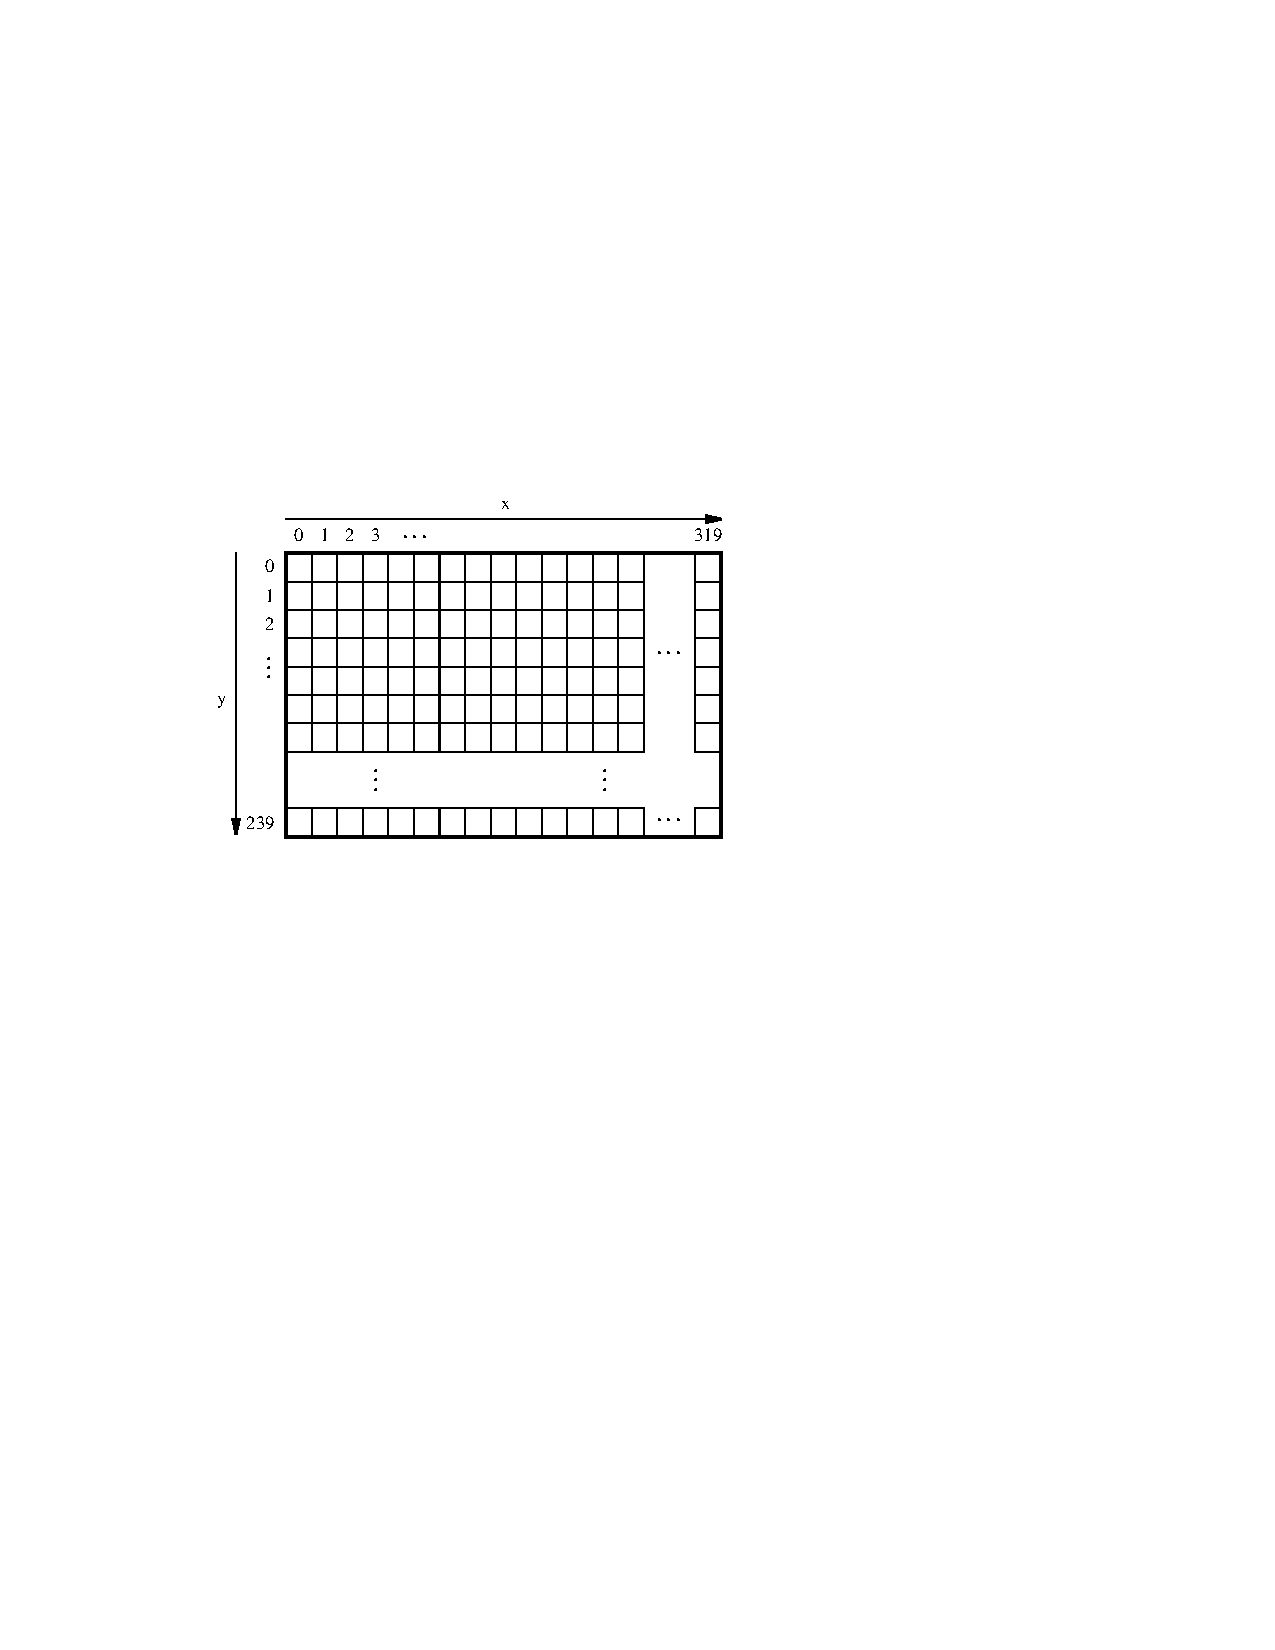
\includegraphics{figures/fig_video_coord.pdf}
   \end{center}
   \caption{Pixel buffer coordinates.}
	\label{fig:video_coord}
\end{figure}

~\\
\noindent
Figure \ref{fig:pixels}$a$ shows that each pixel color is represented as a 16-bit halfword, 
with five bits for the blue and red components, and six bits for green.  As depicted in 
part $b$ of Figure \ref{fig:pixels}, pixels are addressed in the pixel buffer by 
using the combination of a {\it base} address and an {\it x,y} offset. In the computer 
system for your board the default address of the start of the pixel buffer is {\sf 0xC8000000}.
This address corresponds to the beginning of a memory block that is located inside the FPGA
chip in the computer system. Using the addressing scheme in Figure~\ref{fig:pixels}$b$, 
the pixel at location 0,0 has the address {\sf 0xC8000000}, 
the pixel 1,0 has the address {\it base} $+$ (00000000~000000001~0)$_2$ = {\sf 0xC8000002}, 
the pixel 0,1 has the address {\it base} $+$ (00000001~000000000~0)$_2$ = {\sf 0xC8000400}, and 
the pixel at location 319,239 has the address {\it base} $+$ (11101111 100111111 0)$_2$ = 
{\sf 0xC803BE7E}. 

~\\
\noindent
You can create an image by writing color values into the pixel addresses as described
above. A dedicated {\it pixel buffer controller} reads this pixel data from the memory and 
sends it to the VGA display.  The controller reads the pixel data in sequential order, 
starting with the pixel data corresponding to the upper-left corner of the VGA screen and 
proceeding to read the whole buffer until it reaches the data for the lower-right corner. This 
process is then repeated, continuously.  You can modify the pixel data at any time, by writing 
to the pixel addresses. Writes to the pixel buffer are automatically interleaved in the 
hardware with the read operations that are performed by the pixel buffer controller. 

~\\
\noindent
It is also possible to prepare a new image for the VGA display without changing the content 
of the pixel buffer, by using the concept of {\it double-buffering}.  In this scheme two 
pixel buffers are involved, called the {\it front} and {\it back} buffers, as described below.

\begin{figure}[b]
   \begin{center}
       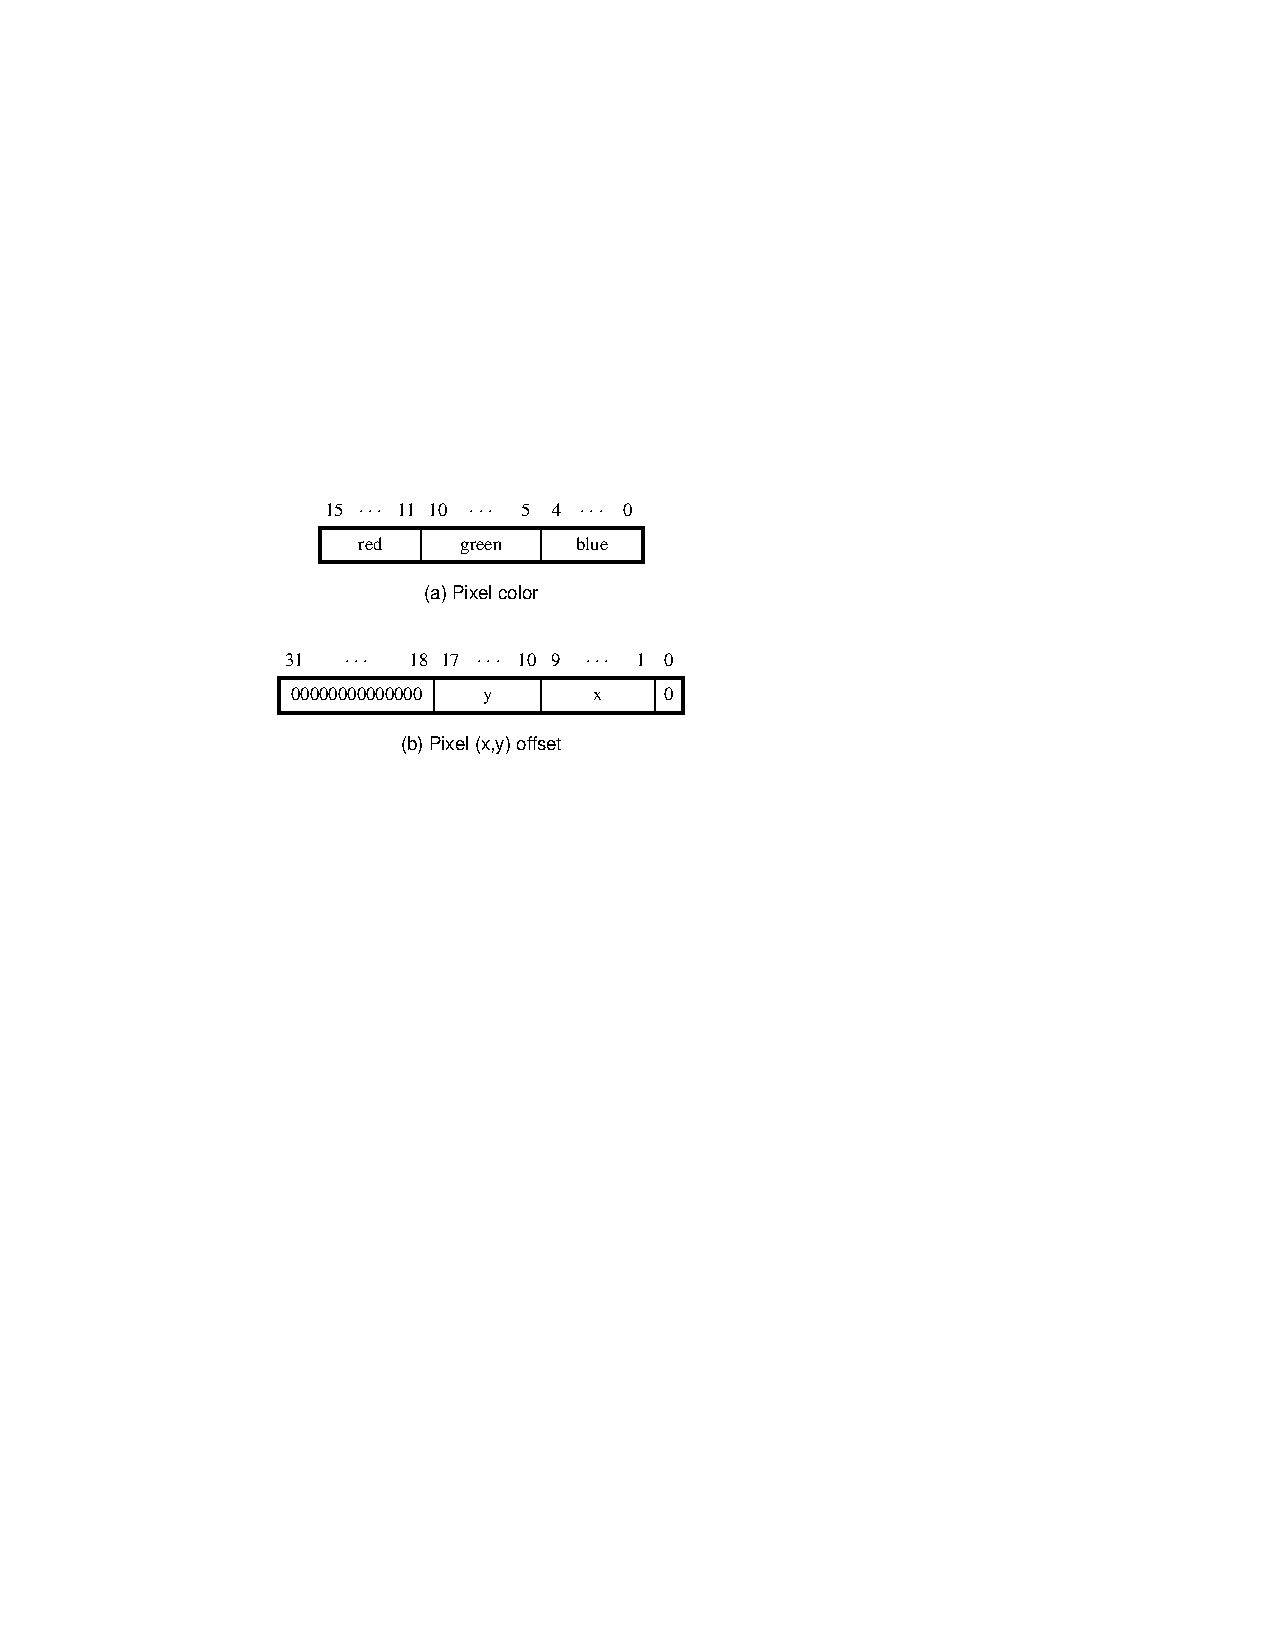
\includegraphics{figures/fig_pixels.pdf}
   \end{center}
   \caption{Pixel values and addresses.}
	\label{fig:pixels}
\end{figure}

~\\
\noindent
{\bf Double Buffering}
\label{sec:double_buffer}

~\\
\noindent
As mentioned above, a pixel buffer controller reads data out of the pixel buffer so that it 
can be displayed on the VGA screen. This pixel buffer controller 
includes a programming interface in the form of a set of registers, as
illustrated in Figure~\ref{fig:pixel_ctrl}. The register at address {\sf 0xFF203020} is called 
the {\it Buffer} register, and the register at address  {\sf 0xFF203024} is the 
{\it Backbuffer} register. Each of these registers stores the starting address of a pixel 
buffer.  The Buffer register holds the address of the pixel buffer that is displayed on
the VGA screen. As mentioned above, in the default configuration of the computer systems the 
Buffer register is set to the address {\sf 0xC8000000}, which points to the start of the FPGA 
on-chip memory.  The default value of the Backbuffer register is also {\sf 0xC8000000},
which means that there is only one pixel buffer. But software can modify the address
stored in the Backbuffer register, thereby creating a second pixel buffer. An image can be
drawn into this second buffer by writing to its pixel addresses. This image is not displayed 
on the VGA monitor until a pixel buffer {\it swap} is performed, as explained below.

~\\
\noindent
A pixel buffer swap is caused by writing the value 1 to the Buffer register. This write
operation does not directly modify the content of the Buffer register, but instead causes
the contents of the Buffer and Backbuffer registers to be swapped. The swap operation does
not happen right away; it occurs at the end of a VGA screen-drawing cycle, after the last 
pixel in the bottom-right corner has been displayed. This time instance is referred to as
the {\it vertical synchronization} time, and occurs every 1/60 seconds. Software can poll the
value of the $S$ bit in the {\it Status} register, at address {\sf 0xFF20302C}, to see when 
the vertical synchronization has happened. Writing the value 1 into the Buffer register
causes $S$ to be set to 1. Then, when the swap of the Buffer and Backbuffer registers 
has been completed $S$ is reset back to 0. The {\it Status} register contains additional bits 
of information, shown in Figure~\ref{fig:pixel_ctrl}. The $m$ and $n$ bits specify the number 
of $y$ and $x$ VGA address bits, respectively. The {\it BS} bits indicate pixel-size; for
a pixel size of two bytes, this field is set to 15. Also, the programming interface includes 
a {\it Resolution} register, shown in the figure, that contains the X and Y resolution of 
the pixel buffer(s).  

\begin{figure}[t]
   \begin{center}
       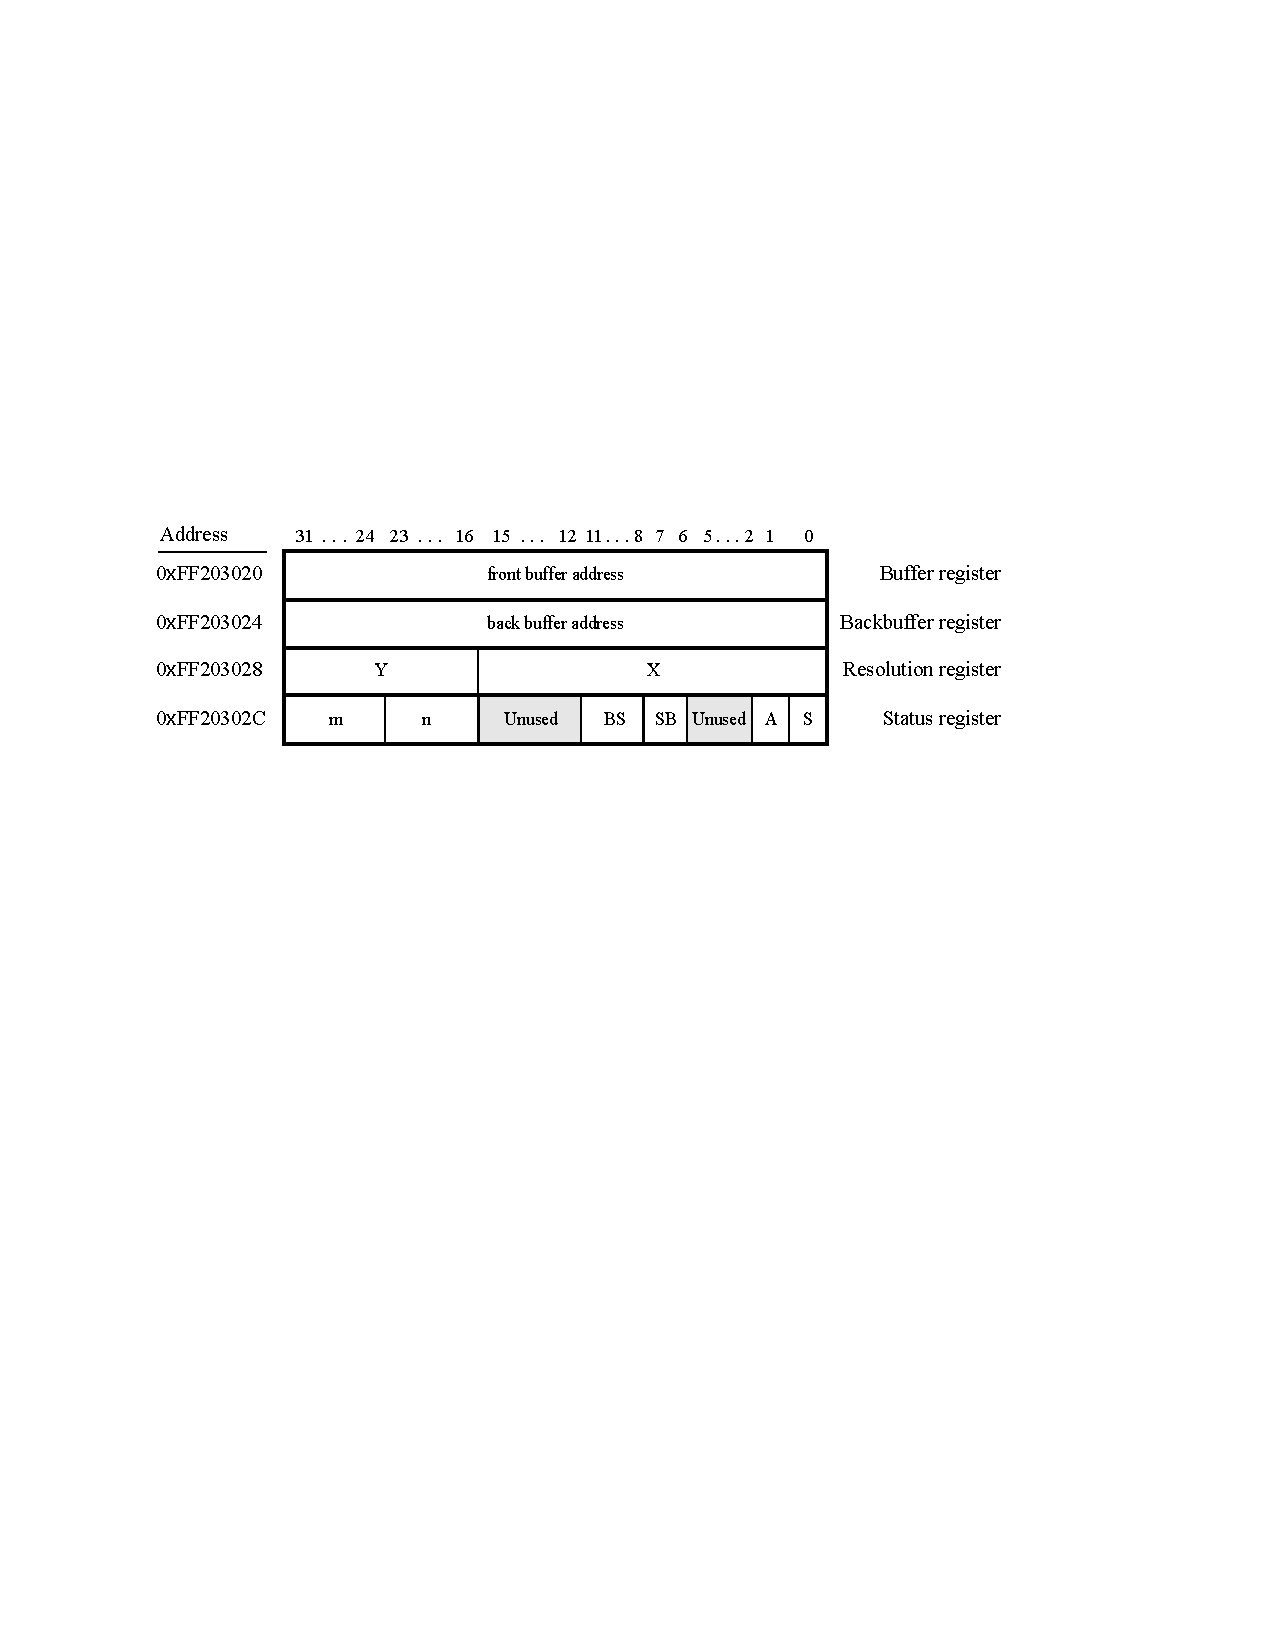
\includegraphics{figures/fig_DMA_ctrl.pdf}
   \end{center}
   \caption{Pixel buffer controller registers.}
	\label{fig:pixel_ctrl}
\end{figure}

~\\
\noindent
In a typical application the pixel buffer controller is used as follows. While the image
contained in the pixel buffer that is pointed to by the Buffer register is being displayed, 
a new image is drawn into the pixel buffer pointed to by the Backbuffer register. When this new
image is ready to be displayed, a pixel buffer swap is performed. Then, the pixel buffer 
that is now pointed to by the Backbuffer register, which was already displayed, is cleared and 
the next new image is drawn. In this way, the next image to be displayed is always drawn into
the ``back'' pixel buffer, and the ``front'' and ``back'' buffer pointers are swapped when 
the new image is ready to be displayed. Each time a swap is performed software has to 
synchronize with the VGA controller by waiting until the $S$ bit in the Status register becomes 0.

~\\
\noindent
{\bf Part I}
~\\
~\\
\noindent
In this part you will learn how to implement a simple line-drawing algorithm.
Drawing a line on a screen requires coloring pixels between two points $(x_1,y_1)$ and 
$(x_2,y_2)$, such that the pixels represent the desired line as closely as possible. Consider 
the example in Figure~\ref{fig:line_drawing}, where we want to draw a line between 
points $(1,1)$ and $(12,5)$. The squares in the figure represent the location and size of pixels
on the screen. As indicated in the figure, we cannot draw the line precisely---we can
only draw a shape that is similar to the line by coloring the pixels that fall closest to 
the line's ideal location on the screen.

\begin{figure}[b]
   \begin{center}
       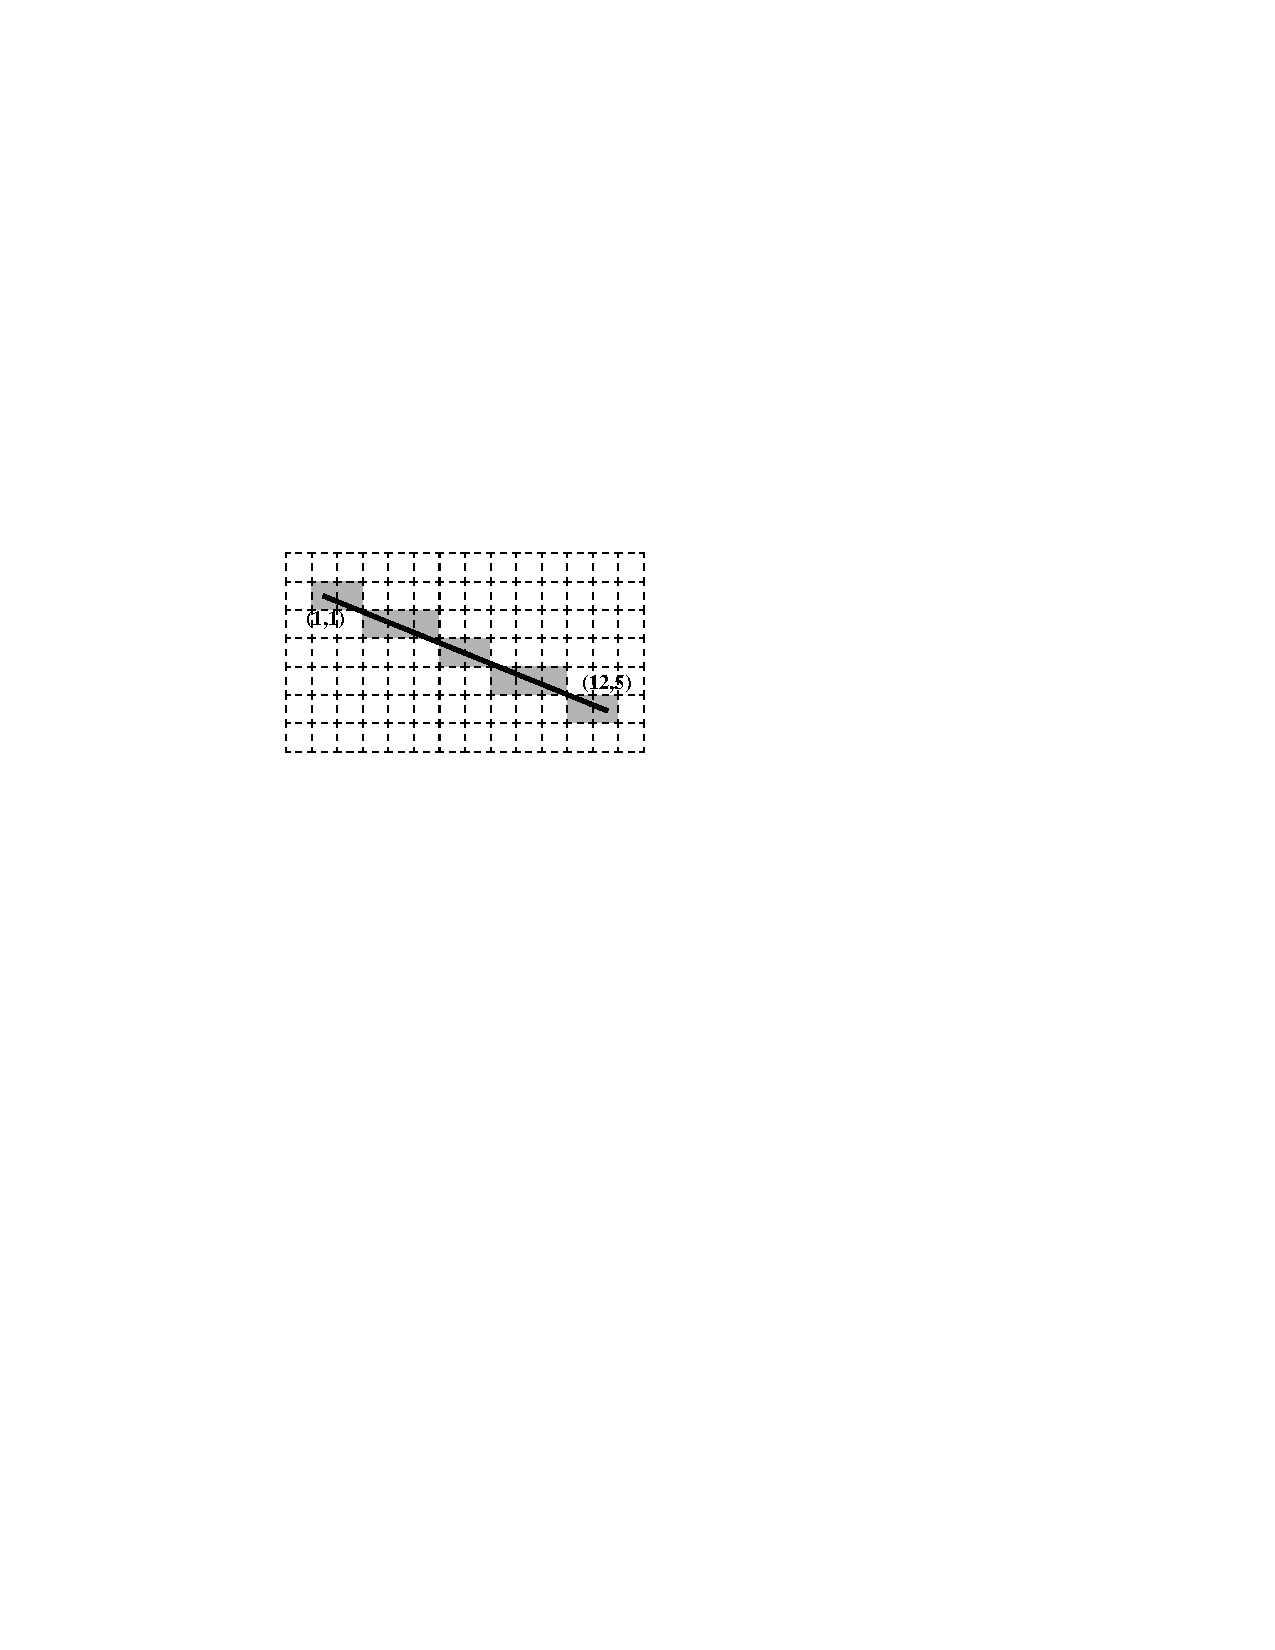
\includegraphics{figures/fig_line_drawing}
   \end{center}
   \caption{Drawing a line between points $(1,1)$ and $(12,5)$.}
	\label{fig:line_drawing}
\end{figure}

~\\
\noindent
We can use algebra to determine which pixels to color. This is done by using the end points and 
the slope of the line. The slope of our example line is $slope = (y_2 - y_1)/(x_2 - x_1) = 4/11$. 
Starting at point $(1,1)$ we move along the $x$ axis and compute the $y$ coordinate for the 
line as follows:

\begin{eqnarray*}
y = y_1 + slope \times (x - x_1)
\end{eqnarray*}

~\\
\noindent
Thus, for column $x = 2$, the $y$ location of the pixel is
$1 + \frac{4}{11} \times (2-1) = 1 \frac{4}{11}$. 
Since pixel locations are defined by integer values we round the $y$ coordinate to the nearest 
integer, and determine that in column $x = 2$ we should color the pixel at $y = 1$. For
column $x = 3$ we perform the calculation $y = 1 + \frac{4}{11} \times (3-1) = 1
\frac{8}{11}$, and round the result to $y = 3$.  Similarly, we perform such computations 
for each column between $x_1$ and $x_2$.

~\\
\noindent
The approach of moving along the $x$ axis has drawbacks when a line is steep. A steep line
spans more rows than it does columns, and hence has a slope with absolute value greater than 
1.  In this case our calculations will not produce a smooth-looking line.  Also, in the case
of a vertical line we cannot use the slope to make a calculation.  To address this 
problem, we can alter the algorithm to move along the $y$ axis when a line is steep. With 
this change, we can implement a line-drawing algorithm known as {\it Bresenham's algorithm}.
Pseudo-code for this algorithm is given in Figure~\ref{fig:line_algorithm}. The first 15
lines of the algorithm make the needed adjustments depending on whether or not the line is
steep, and on its vertical (down or up) and horizontal (left or right) directions.
Then, in lines 17 to 25 the algorithm increments the {\it x} variable 1 step at a time
and computes the {\it y} value. The {\it y} value is incremented when needed to stay as
close to the ideal location of the line as possible. Bresenham's algorithm calculates an
{\it error} variable to decide whether or not to increment each {\it y} value.
The {\it error} variable takes into account the relative difference
between the width ({\it deltax}) and height of the line ({\it deltay}) in deciding
how often {\it y} should be incremented. The version of the algorithm shown in 
Figure~\ref{fig:line_algorithm} uses only integers to perform all calculations. 

\begin{figure}[H]
\centering
\begin{lstlisting}[language=C, numbers=left, stepnumber=1, xleftmargin=1cm,
morekeywords={then}]
  draw_line(x0, x1, y0, y1)
		
		boolean is_steep = abs(y1 - y0) > abs(x1 - x0)
		if is_steep then
			swap(x0, y0)
			swap(x1, y1)
		if x0 > x1 then
			swap(x0, x1)
			swap(y0, y1)
			
		int deltax = x1 - x0
		int deltay = abs(y1 - y0)
		int error = -(deltax / 2)
		int y = y0
		if y0 < y1 then y_step = 1 else y_step = -1
		
		for x from x0 to x1
			if is_steep then 
				draw_pixel(y, x)
			else 
				draw_pixel(x, y)
			error = error + deltay
			if error >= 0 then
				y = y + y_step
				error = error - deltax
			
\end{lstlisting}
\caption{Pseudo-code for a line-drawing algorithm.}
\label{fig:line_algorithm}
\end{figure}

~\\
\noindent
Perform the following:

\begin{enumerate}

\item Write a C-language program that implements Bresenham's line-drawing algorithm,
and uses this algorithm to draw a few lines on the screen.  An example of a suitable main 
program is given in Figure~\ref{fig:main1}. The code first determines the address of the 
pixel buffer by reading from the pixel buffer controller, and stores this address into the
global variable {\it pixel\_buffer\_start}. The main program clears the screen, and then 
draws four lines.  An example of a function that uses the global variable 
{\it pixel\_buffer\_start} is shown at the end of Figure~\ref{fig:main1}. The function 
{\it plot\_pixel ()} sets the pixel at location {\it x}, {\it y} to the color {\it line\_color}. 
This function implements the pixel addressing scheme from Figure~\ref{fig:pixels}$b$.

\item Create a new Monitor Program project for your DE-series board computer to use 
		  with your C code.

\item Connect a VGA monitor to your DE-series board, and compile and run your program.
\end{enumerate}

\begin{figure}[H]
\centering
\lstinputlisting[language=C]{../design_files/part1.c}
\caption{Part of the program for Part I.}
\label{fig:main1}
\end{figure}

~\\
\noindent
{\bf Part II}

~\\
\noindent
Animation is an exciting part of computer graphics. Moving a displayed object is an illusion 
created by showing this same object at different locations on the screen. A simple way to
``move'' an object is to first draw the object at one position, and then after a short time erase 
the object and draw it again at another nearby position. To realize animation it is necessary 
to move objects at regular time intervals. The VGA controller in your DE-series board's computer 
system redraws the screen every $1/60^{th}$ of a second. Since the image on the screen cannot 
change more often than that, it is reasonable to control an animation using this unit of time.

~\\
\noindent
To ensure that the VGA image is changed only once every $1/60^{th}$ of a second, you can use the 
pixel buffer controller to synchronize with the vertical synchronization cycle of the VGA 
controller. As we discussed in the background section of this exercise, synchronizing with the 
VGA controller can be accomplished by writing the value 1 into the {\it Buffer} register in the 
pixel buffer controller, and then waiting until bit $S$ of the {\it Status} register becomes 
equal to 0. For this part of the exercise you do not need to use a back buffer, so ensure
that the {\it Buffer} and {\it Backbuffer} addresses in the pixel buffer controller are the 
same. In this approach, a pixel buffer ``swap'' can be used as a way of synchronizing with 
the VGA controller via the {\it S} bit in the {\it Status} register.

~\\
\noindent
Perform the following:

\begin{enumerate}

\item Write a C-language program that moves a horizontal line up and down on the screen and 
``bounces'' the line off the top and bottom edges of the display. Your program should first 
clear the screen and draw the line at a starting row on the screen. Then, in an endless
loop you should erase the line (by drawing the line using black), and redraw it one row
above or below the last one.  When the line reaches the top, or bottom, of the screen 
it should start moving in the opposite direction.

\item Make a new Monitor Program project to test your code. Notice how long it takes for the 
horizontal line to move through the 240 lines of the VGA display. It should take 
$240 \times 1/60 = 4$ seconds.
\end{enumerate}

~\\
~\\
\noindent
{\bf Part III}
~\\

\noindent
Having gained the basic knowledge about displaying images and animations, you can now create 
a more interesting animation.

~\\
\noindent
You are to create an animation of eight small filled rectangles on the screen. These rectangles 
should appear to be moving continuously and ``bouncing'' off the edges of the screen. The 
rectangles should be connected with lines to form a chain. An illustration of the animation 
is given in Figure~\ref{fig:animation_example}. Part $a$ of the figure shows one position
of the rectangles with arrows that indicate the directions of movement, and 
Figure~\ref{fig:animation_example}$b$ shows a subsequent position of the rectangles. 
In each step of your animation each of the rectangles should appear to ``move'' on a diagonal 
line: up/left, up/right, down/left, or down/right. Move the rectangles one
row and one column at a time on the VGA screen.

\begin{figure}[h!]
   \begin{center}
       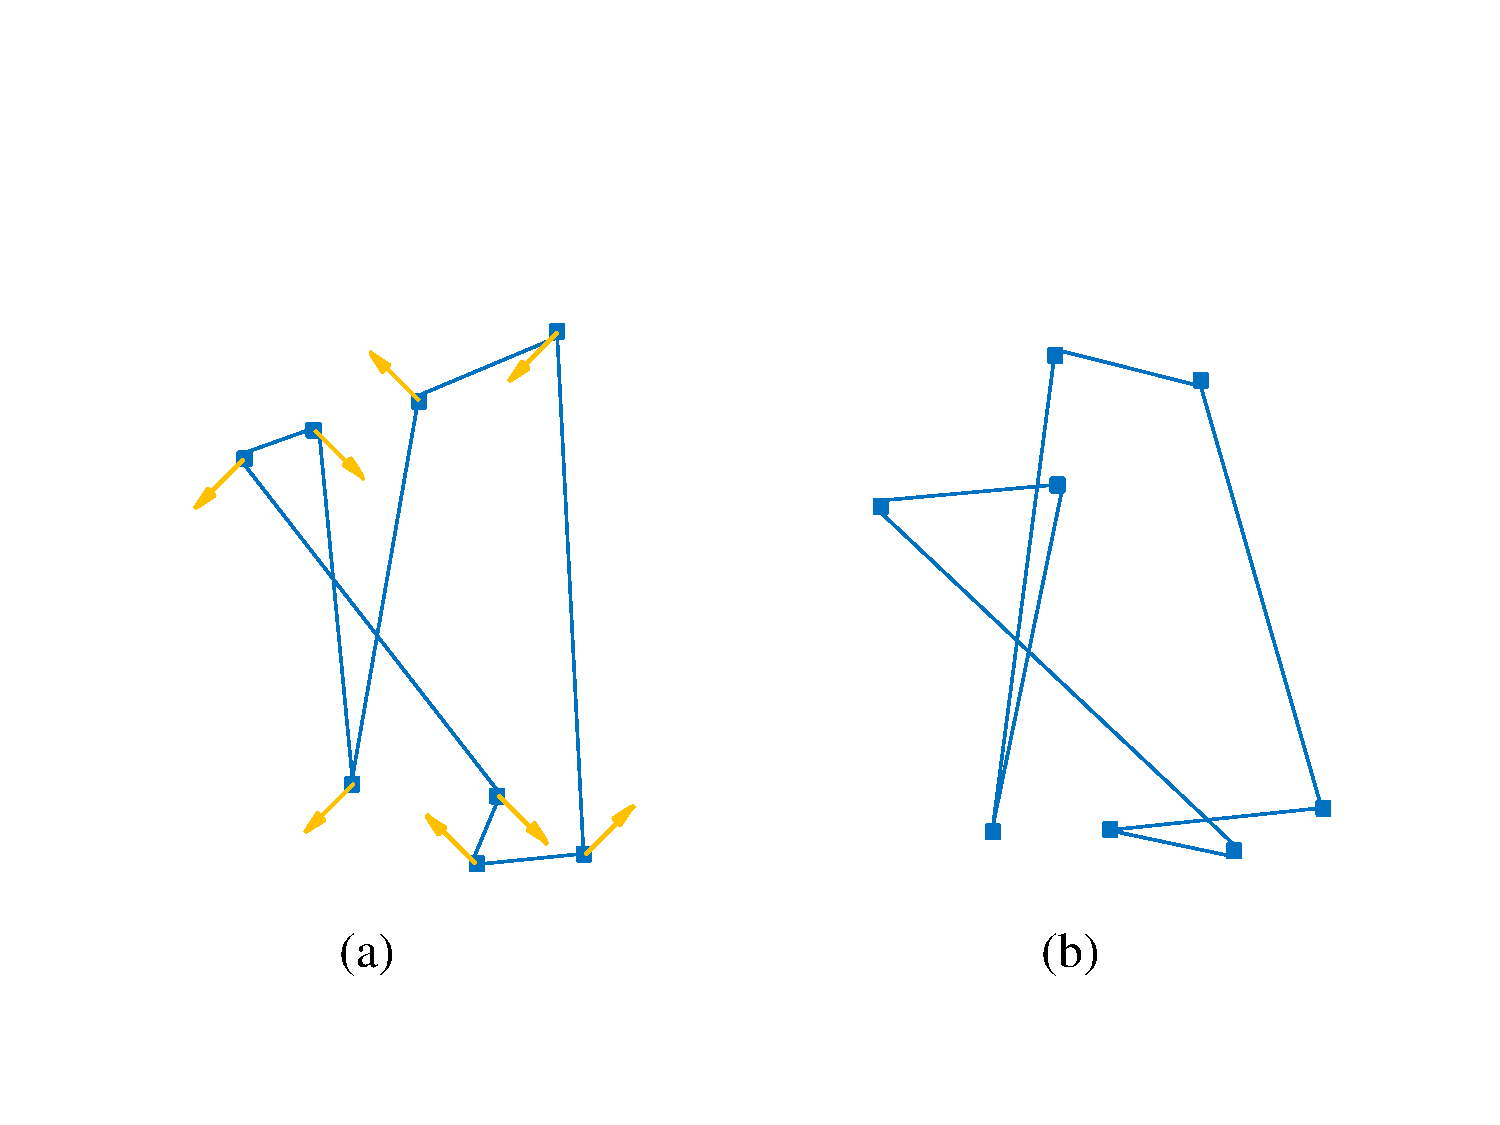
\includegraphics[scale = 0.5]{figures/fig_animation_example.pdf}
   \end{center}
   \caption{Two instants of the animation.}
	\label{fig:animation_example}
\end{figure}

~\\
\noindent
To make the animation look slightly different each time you run it, use the C library function 
{\it rand ()} to help calculate initial positions for each of the rectangles, and to determine 
their directions of movement. 

~\\
\noindent
Perform the following:

\begin{enumerate}

\item Write a C-language program to implement your animation. Use both a front and back buffer 
in your program, so that you can avoid making changes to the image while it is being displayed 
by the pixel buffer controller.  An example of a suitable main program is given in 
Figure~\ref{fig:main3}. The code sets the location in memory of both the front and back pixel 
buffers---the front buffer is set to the start of the FPGA on-chip memory, and the back
buffer to the starting address of the {\it SDRAM} memory that is included on your the DE-series
board. In each iteration of the while loop the code clears the entire screen, 
draws the rectangles and lines, and then 
updates the locations of rectangles. At the bottom of the while loop the code calls the
function {\it wait\_for\_vsync ()}, which synchronizes with the VGA controller and swaps the 
front and back pixel buffer pointers.

\item Make a new Monitor Program project to test your code.

\item Experiment with your code by modifying it to use just a single pixel buffer (simply
change the address of the back buffer to be the same as the front buffer). Explain what you 
see on the VGA screen as a result of this change.
\end{enumerate}

\begin{figure}[H]
\centering
\lstinputlisting[language=C]{../design_files/part3.c}
\caption{Main program for Part III.}
\label{fig:main3}
\end{figure}

\newpage
\noindent
{\bf Part IV}

\noindent
~\\
For this part of the exercise you are to enhance the animation from Part~III so that
during the animation the following changes can take place:

\begin{enumerate}
\item
The speed of movement of the rectangles can increased or decreased
\item
The number of rectangles can be increased or decreased
\item
The lines between rectangles can be drawn or not drawn
\end{enumerate}

~\\
\noindent
In Part III the speed of animation was set by the 1/60 seconds VGA vertical synchronization time.
One way to control the speed of animation is to make use of a timer. In this scheme, the main 
program would draw the next step of the animation each time the timer expires.  Lengthening 
the timeout would produce a slower animation, and shortening the timeout would speed up the 
animation. The maximum speed 
of the animation would be limited by the 1/60 seconds VGA synchronization time, as it was in 
Part III.  To cause the animation to appear to move more quickly than in Part III, you
have to increase the screen-distance that the rectangles move in each step of the animation.

~\\
\noindent
Perform the following:

\begin{enumerate}

\item Implement the speed control discussed above for the animation. The speed of animation 
should approximately double when you press pushbutton {\it KEY}$_0$, and it should reduce by 
the same amount when you press {\it KEY}$_1$. Pressing {\it KEY}$_2$ should cause the
program to display one fewer rectangle, down to a minium of one, and pressing {\it KEY}$_3$
should increase the number of rectangles to some maximum of your choosing. You can process
the pushbutton {\it KEYs} using either polled I/O or using interrupts. Finally, when
any slide switch {\it SW}$_{9-0}$ is set to the 1 position the lines between rectangles should 
not be drawn; only when all {\it SW} switches are set to the 0 position should the lines appear.

\item Make a new Monitor Program project to test your code.

\item Add any other animation features that you may find interesting.
\end{enumerate}

\section*{Part V}

\noindent
We mentioned earlier in this exercise that the image displayed by the VGA
controller can be derived from two sources: the pixel buffer, which displays graphics, 
and a {\it character} buffer, which displays text. For this part of the exercise you 
are to enhance your code so that it supports the display of text. The character buffer 
is stored in FPGA on-chip memory in the DE1-SoC Computer. Figure \ref{fig:chars}$a$ 
depicts the character buffer for the VGA
display, which has a resolution of 80 $\times$ 60 characters. Each character occupies an
8 $\times$ 8 block of pixels on the screen. Characters are stored in each of the locations
shown in Figure \ref{fig:chars}$a$ using their ASCII codes; when you store an ASCII character into
the buffer, a corresponding pattern of pixels is automatically generated and displayed using 
a built-in font. Part~$b$ of Figure~\ref{fig:chars} shows
that characters are addressed in the memory by using the combination of a {\it base} address,
which has the value (C9000000)$_{16}$, and an {\it x,y} offset. Using this scheme, the
character at coordinates $(0,0)$ has the address (C9000000)$_{16}$, 
$(1,0)$ has the address {\it base} $+$ (000000 0000001)$_2$ = (C9000001)$_{16}$, 
$(0,1)$ has the address {\it base} $+$ (000001 0000000)$_2$ = (C9000080)$_{16}$, and 
the character at location $(79,59)$ has the address {\it base} $+$ (111011 1001111)$_2$ = 
(C9001DCF)$_{16}$. 

\begin{figure}[h]
   \begin{center}
       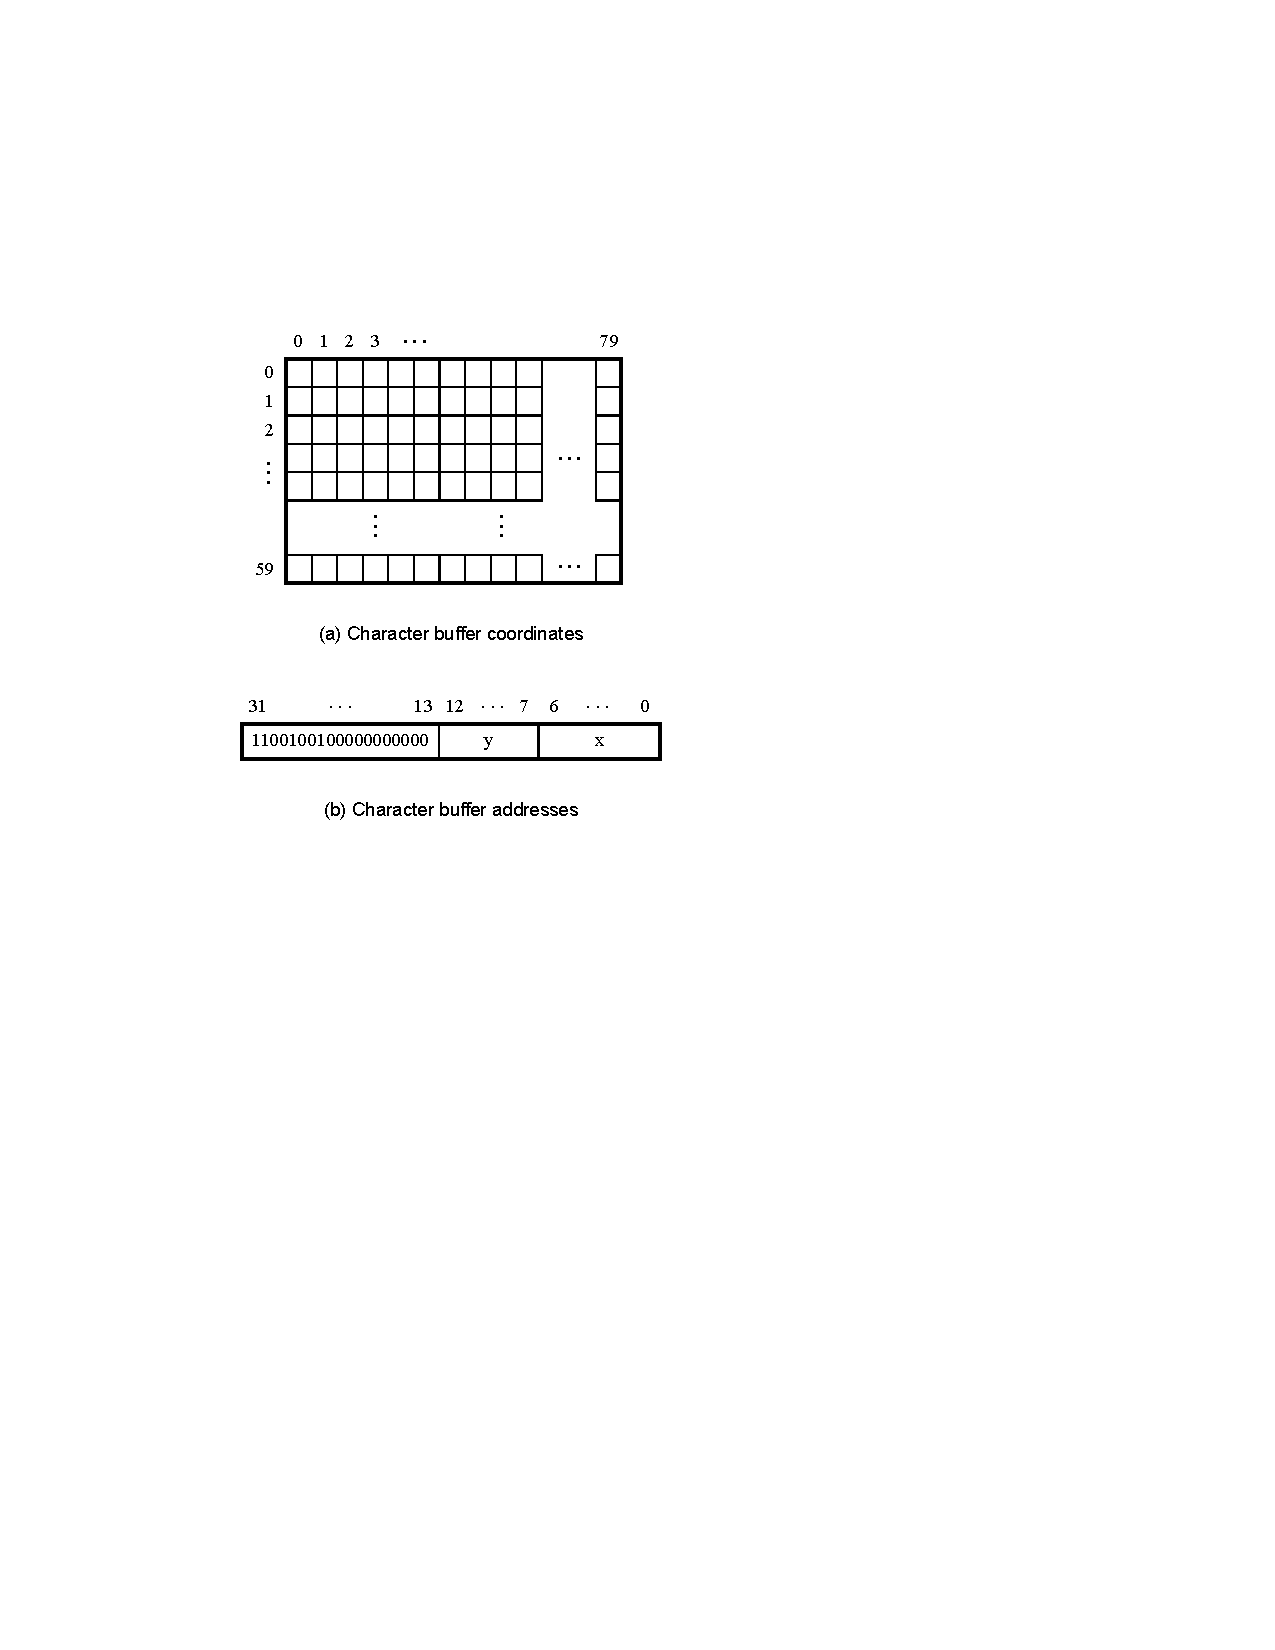
\includegraphics{figures/fig_chars.pdf}
   \end{center}
   \caption{Character buffer coordinates and addresses.}
	\label{fig:chars}
\end{figure}

~\\
\noindent
The character buffer has an associated controller, with a
register interface like the one shown in Figure~\ref{fig:pixel_ctrl}. You can read from the
{\it Resolution} register to obtain the number of text columns ($X$) and rows ($Y$) on
the screen. For the VGA screen, the values will be 80 columns $\times$ 60 rows.

~\\
\noindent
Perform the following:

\begin{enumerate}
\item Enhance your solution code from Part IV so that it can display text on the VGA screen. 
Your code should be able to clear all characters from the VGA screen (by filling the
character buffer with the `~' space character). Your code should be able to store an ASCII 
string into the coordinates starting at \texttt{(x, y)} in the character buffer. 
\item As an example of using the character buffer, augment your program from Part IV so that 
it displays, in the upper-left corner of the screen, the number of video frames that have 
been drawn. Using the default animation speed, which is determined by the VGA vertical 
synchronization time, the frame counter should increment at the rate of 60 times per second.
\item Compile and test your animation.
\end{enumerate}

%%%%%%%%%%%%%%%%%%%%%%%%%%%%%%%%%%%%%%%%
%%% FPGAcademy Copyright Information %%%
%%%%%%%%%%%%%%%%%%%%%%%%%%%%%%%%%%%%%%%%

%Always put the copyright on a new page (clear page), with some vertical space from top
\clearpage
\vspace{1in}

\noindent

Copyright {\copyright} FPGAcademy.org. All rights reserved. FPGAcademy and the 
FPGAcademy logo are trademarks of FPGAcademy.org.  This document is provided 
"as is", without warranty of any kind, express or implied, including but not 
limited to the warranties of merchantability, fitness for a particular purpose 
and noninfringement. In no event shall the authors or copyright holders be 
liable for any claim, damages or other liability, whether in an action of 
contract, tort or otherwise, arising from, out of or in connection with the 
document or the use or other dealings in the document.
~\\
~\\
**Other names and brands may be claimed as the property of others.


\end{document}
